%! Author = erick-hdz
%! Date = 15/05/20

% Preamble
\documentclass[10pt]{report}


% Packages
\usepackage{blindtext}
\usepackage{amsmath}
\usepackage[utf8]{inputenc}
\usepackage[spanish]{babel}
\usepackage{fancyhdr}
\usepackage{graphicx}
\usepackage{algorithm, algorithmic}
\usepackage{amsfonts}
\usepackage{amsbsy}
\usepackage{makeidx}
\usepackage{geometry}
\usepackage{listings}
\usepackage[T1]{fontenc}
\usepackage{natbib}
\usepackage{amsthm}
\usepackage{amssymb}
\usepackage{lastpage}
\usepackage{multicol}
\usepackage{xcolor}

%Status of the document

\pagenumbering{roman}
\newtheorem{example}{Example}
\newtheorem{corrollary}{Corrollary}
\newtheorem*{remark}{Remark}
\newtheorem{definition}{Definition}
\newtheorem{theorem}{Theorem}
\pagestyle{fancy}
\fancyhf{}
\rhead{Sección de tesis}
\lhead{Simulación de modelos}
\rfoot{Page  \thepage}
\author{Erick Hernandez Navarrete}
\title{Simulación de modelos}


% Document
\begin{document}
    %todo:Correcciones del documento en forma de check speller
    %todo:Hacer antes de esta semana lo antes posible
    %todo:puntear a manera de commit los elementos del Cap 1
    %TODO:Hacer las correcciones de al menos el primer capitulo de la tesis
    \maketitle
    \tableofcontents{}
    \chapter{Decidibilidad en los modelos}\label{ch:decidibilidad-en-los-modelos}
    \section{Introducción}\label{sec:introducción}
    En este documento se expondrán las nociones de decibilidad, complejidad en ambos modelos %Add complexity part of both worlds
    en el mundo de máquinas de Turing y en el mundo distribuido,
    así como también se hará la formalización de la noción de simulación de modelos
    computacionales, demostrando que el modelo $A$ de  la máquina de
    Turing es equivalente en poder al modelo distribuido $B$, en particular al modelo \textbf{LOCAL}

    \section{Decidibilidad en el modelo de máquinas de Turing}\label{sec:decidibilidasd-en-el-modelo-de-máquinas-de-turing}
    %!todo:Hacer una explicacion intuitiva de lo que es una máquina de Turing,despues de esta done
    %!todo: de esta explicación intuitiva
    %!todo: Hacer un feedback con la escritura para que se pula la parte de la gramática


    \subsection{Cadenas y lenguajes}\label{sec:Cadenas-y-lenguajes}
    Ahora, se definirán los bloques constructores de ciencias de la computación, es decir las cadenas de carácteres.
    Con el propósito de definir lo siguiente:\space
    \begin{definition}
            Decimos que un alfabeto es cualquier conjunto $X$ tal que $X != \emptyset$
    \end{definition}
    \newline
    Una vez que se define el concepto de alfabeto, los elementos del lenguaje son los símbolos del alfabeto.
    Se estipulará que las letras mayúsculas se usarán para los alfabetos y letras minúsculas para los símbolos.
    En virtud de ello se pude enuciar algunos ejemplos de alfabetos:
    \begin{itemize}
        \item $\Theta_{1} = \{0,1,2,3,4,5,6,7,8,9 \}$
        \item $\Theta_{2} = \{a,b,c,d,e,f,g,h,i,j,k,l \}$
        \item $\Omega = { 0,1,x,y,z,t}$
    \end{itemize}\space
    Lo siguiente es definir la noción de una cadena sobre un alfabeto, que para los fines de este estudio
    son los bloques constructores del mismo, y que son, al mismo tiempo, en el modelo de
    máquinas de Turing las entradas de instancias de este modelo, lo que dará la noción de cómputo.
    \begin{definition}
        Una \textbf{cadena} sobre un alfabeto $\Sigma$ es una secuencia finita de símbolos del alfabeto,
       que es usualmente escrito cada símbolo uno sobre otro y sin separación por comas.
    \end{definition}
    Una vez que se tiene la noci ón de cadena sobre un alfabeto, se puede dar unos cuantos ejemplos:
    \begin{itemize}
        \item Si $\Sigma_{1} = \{a,b\}$, entonces la cadena $abbaba$ es una cadena sobre $\Sigma_{1}$
        \item Si $\Sigma_{2} = \{ 2,3,5 \}$, entonces la cadena $32225$ es una cadena sobre $\Sigma_{2}$
    \end{itemize}
    Entonces ahora que se definió el concepto cadena sobre un alfabeto podemos definir atributos a las cadenas definidas sobre un
    alfabeto $\Sigma$,\newline
    \begin{definition}
        Sea $w$ una cadena sobre un alfabeto $\Sigma$,dicha cadena tiene \textbf{longitud},
        y se denotorá como $|w|$, y asi se concluirá que es el número de símbolos que contiene.

    \end{definition}
    Entonces con base a esa definición, se denominará vacía a la cadena tal que su longitud es cero, y la
    distinguiremos como $\epsilon$.\newline
    Se puede escribir a una cadena $w = w_{1},\mathellipsis w_{n}$, sobre un alfabeto $\Sigma$ si cada $w_{i} \in \Sigma$;
    \space
    A continuación se definirán ciertas operaciones o atributos asociados a estas estructuras de datos.
    \begin{definition}
        Sea una cadena $w$, se asociará a la cadena $w$ la cadena reversa denotada como $w^R$
        y con la notación, si $w = w_{1},\mathellipsis w_{n}$, entonces $w^{R} = w_{n},\mathellipsis,w_{1}$.
    \end{definition}
    También se dará la noción de sub-cadena, la cual enunciaremos de la siguiente manera:\newline
    \begin{definition}
        Sean $z,w$ cadenas, se puede decir que $z$ es una sub-cadena de $w$ si aparece de manera consecutiva dentro de $w$.
    \end{definition}
    Ejemplos de subcadenas son:
    \begin{itemize}
        \item $abc$ es una sub-cadena de la cadena $abcdedfg$
        \item $cdcd$ es una subcadena de la cadena $cdasdcadccdcd$
    \end{itemize}
    También se definirá una operación entre dos cadenas, la cual es
    la concatenación, entonces se define formalmente de la siguiente manera:\newline
    \begin{definition}
        Sean $w_{1}$ y $w_{2}$ dos cadenas finitas, esto es:\newline
        $\exists n,\ \exists m$ tal que $|w_{1}|=n$ y $|w_{2}|=m$
        entonces la cadena $r = w_{1}w_{2}$, es el resultado de agregar la cadena $w_{2}$ al final de la cadena
        $w_{1}$.\newline
        En notacion es: $concat(w_{1},w_{2}) = w_{1}w_{2}$
    \end{definition}
    Entonces con esta definición de operación se hará el equivalente en potencia en matemáticas,
    formalmente lo podemos decir:\newline
    \begin{definition}
        Sea $x$ una cadena sobre un alfabeto $\Sigma$, entonces concatenar dicha cadena
        $m-veces$, con $m\in\N$ se escribirá así:\newline
        $x\dots x = x^m$
    \end{definition}
    Finalmente se tiene los terminos "universo" de las cadenas para algún alfabeto, que se formalizará de la
    siguiente manera:
    \begin{definition}
        Sea un alfabeto $\Sigma$, se dice que un lenguaje es un conjunto de cadenas sobre el alfabeto $\Sigma$, i.e
        \begin{equation}
            \label{eq:equation7}
             L = \{w : w\ es \ una \ cadena\ sobre \Sigma \}
        \end{equation}
    \end{definition}
    Entonces, una vez que se tiene la definición de lenguaje, lo siguiente es presentar el modelo de máquina de Turing,
    ya que en este contexto los problemas se modelarán en términos de lenguaje, con la noción anteriormente anunciada.


    \subsection{Elementos del modelo}\label{subsec:elementos-del-modelo-de-máquina-de-turing}
    Ahora, se dará la definición del modelo formal de computo, a saber el modelo de máquina de Turing,
    para ello se tendrá una presentación intuitiva del modelo.\newline
    El modelo de máquina de Turing es a grandes razgos un modelo acaparable; lo cual quiere decir, se tendrá la posiblidad
    de resolver una cantidad de problemas, pero con ciertas limitantes.
    \space

    Este modelo fue propuesto por primera vez en 1936 por el matemático \textbf{Alan Turing} similares a
    otros modelos de cómputo que no se presentará en esta tesis, como son solo por decir: autómatas finitos.
    El modelo de máquina de Turing usa una cinta infinita como su memoria ilimitada,
    además tine el cabezal, que es la que permité leer y escribir símbolos además de moverse
    a lo largo de la cinta.
    \space
    Inicialmente la cinta contiene únicamente como entrada a la cadena, y lo demás es blanco.
    Si la máquina necesita almacenar información que tendrá que ser escrita en la cinta.
    Para leer la información que ha sido escrita en la cinta esta tendrá que mover su cabezal sobre ella.\space
    La máquina continurá computando hasta que tenga una salida, lo que se traduce a que tendrá una sucesión de pasos
    como los que se describieron anteriormente, hasta que se dé la definición formal de la palabra cómputo.
    \space

    Las salidas "aceptación, rechazo" se obtienen una vez que se ha entrado en los estados de "aceptacion, rechazo",
    por otro lado si no entrá en alguno de los estados que se mencionaron anteriormente, la máquina continurá para siempre, i.e
    ésta nunca terminará de hacer su cómputo.\space
    Esta es la presentación intuitiva de este modelo, entonces lo que sigue es definir de manera formal los elementos del modelo,


    \begin{definition}%!Here we need to rewrite for errors
        Una máquina de Turing is una 7-tupla, $(Q,\Sigma,\Lambda,\delta,q_{0},q_{accept},q_{reject})$
        donde $Q,\Sigma,\Lambda$ son conjuntos finitos.
        \begin{enumerate}
            \item $Q$ es el conjunto de estados,
            \item $\Sigma$ es el alfabeto de entrada que no contiene el símbolo blanco $\sqcup$
            \item $\Lambda$ es el alfabeto de la cinta donde  $\sqcup\in\Lambda$ y además $\Sigma\subseteq\Lambda$,
            \item $\delta: Q\times\Lambda \rightarrow Q\times\Lambda\times\{L,R,S\}$ es la función de transición
            \item $q_{0}$ es el estado de iniciación,
            \item $q_{accept}$ es el estado de aceptacion
            \item $q_{reject}$ es el estado de rechazo donde $q_{accept} \neq q_{reject}$,

        \end{enumerate}
        Aquí los símbolos $L,R,S$ son el imperativo para el movimiento del cabezal \textbf{Left}, \textbf{Right} y \textbf{Stay}
    \end{definition}
    Una vez que se tiene la definición se presentará como es el cómputo:\newline
    Inicialmente, se tendrá como entrada una cadena $w = w_{1}\dots w_{n}$ en $\Sigma$, en a lo más $n$ cuadros
    a la izquierda y el resto de la cinta esta en blanco.Ésto quiere decir que están rellenados con símbolos blancos,
    y la manera de identificar el final de la entrada $w$ es marcado por el primer símbolo en blanco en la cinta,
    ya que el alfabeto $\Sigma$ no contiene dicho símbolo.
    \space

    Luego, una vez que inicia la máquina $M$ con la entrada $w$, el cómputo estará gobernado por la función $\delta$.
    Algo que se puede observar es que si en algún momento del cómputo el cabezal intenta moverse a la izquierda del lado
    izquierdo extremo, éste se quedará en el mismo lugar, aunque la función de transición indique un movimiento del cabezal $L$.

    \space
    Finalmente, el cómputo continuará hastá que entre en el estado de $q_{accept}$ ó $q_{reject}$,
    si no sucede lo anterior $M$ continuará para siempre.
    Una vez presentado el modelo y una visión intuitiva del cómputo en el mismo, se adentrará a la noción de
    \textbf{decidible}, que es la noción a la que se quiere converger en este modelo para hacer la conexión con el modelo
    de cómputo distribuido.

    \newspace
    %!todo:Definir como se estan resolviendo los problemas en el contexto de maquinas de Turing
    %!todo:Esto quiere decir que es un lenguaje etc.
    %!Final de las observaciones de la edicion de este capitulo.
     \subsection{Decidibilidad}\label{subsec:decidibilidad2}
    Ahora la noción de \textbf{configuración} es lo que nos permitirá formalizar el movimiento del
    cabezal de la máquina, que esto en esencia será la formalización del cómputo en este modelo.
    \newline
    La manera en que $M$ hace el compúto, de manera intuitiva se puede decir que ocurren ciertos eventos, a saber:
    \begin{itemize}
        \item Cambio en el estado actual
        \item Cambio en el contenido de la cinta
        \item Cambio en la localidad del cabezal
    \end{itemize}
    Estos eventos se constituirán al definir el término configuración.
    Los elementos serán en esencia tomarse el estado actual, digamos $q_{a}$, el contenido actual de la cinta, por ejemplo:
    $uv$ con $u,v$ cadenas para el alfabeto $\Sigma$ y la localidad actual de la cinta, que será el primer
    símbolo de la cadena $v$. \newline
    Esto se puede plantear en la triada:
    \begin{equation}
        C = (u,q,v)
    \end{equation}
    Con $u,v$ cadenas y $q$ es el estado actual, y la posición actual es el primer símbolo de la cadena $v$,
    en este sentido se puede escribir de la siguiente manera esta noción:
    \begin{equation}
        uqv
    \end{equation}
    Para enfatizar que en ese momento del compúto, el cabezal esta en la localidad del primer símbolo de la cadena
    $v$, se coloca a el estado actual $q$ entre la cadena $u$ y $v$; esto da un significado formal a la notación del concepto
    de configuración.
    \\
    \newline
    Entonces esta noción es la que va a dar el paso de formalizar el compúto, por lo cual de manera intuitivamente se va
    a tener una secuencia de configuraciones:
    \begin{equation}
        C_{0}\mathellipsis C_{n}, n\in \N
    \end{equation}
    Pero este proceso se definirá entre dos estados a priorí $C_{i},C_{j}$;
    entonces esta noción permitirá definir lo siguiente:
    \begin{definition}
        Se dice que la \textbf{configuración} $C_{j}$ le sigue a $C_{k}$ si:
        Se toman las cadenas $u,v$ de $\Gamma$, y también $a,b\in \Sigma$.
        entonces se concluye que: si pasa $\delta(q_{k},b) = (q_{j},c,L)$,
        entonces $uacq_{j}v$ le sigue de $uaq_{k}bv$

    \end{definition}
    La anterior noción se esta definiendo con la función $\delta$, que es la que esta formalizando esta noción.
    Como se menciono anteriormente, se estipula que las secuencias de configuraciónes, entonces se tendrá una configuración
    inicial.
    \begin{definition}
        Sea $M$ una máquina de Turing, $w$ una cadena,
        a la configuracion inicial $C_{0}$ la representaremos con base a lo anterior como $q_{0}w$
        \end{definition}
    El significado de la notación de la configuración inicial es que esta en
    el estado cero $q_{0}$ y el cabezal esta en el primera localidad de lado izquierdo de la cinta.
    Ahora las configuraciones que intuitivamente son las candidatas para
    que sean las configuraciones finales si es que la máquina termina en algun momento de este
    proceso; pero por el momento se llamará a esas configuraciones:\newline
    \begin{equation}
        q_{accept}, q_{reject}\label{eq:equation8}
    \end{equation}
    A estas configuraciones se les nombrarán como configuraciones de paro, ya que están definidas
    en términos del estado en el que entran; que son los estado de paro y de aceptación respectivamente.
    %TODO: Hacer una revisión gramatical de la tesis
    Entonces se puede formalizar que una máquina de Turing se detiene si entra en los estados
    $q_{accept0},q_{reject}$ y con base a esto se hace eneralización de la función delta tomando
    un conjunto de estados en el que no esta los estado de detención
    \newline
    Una vez aclarado esto, se tienen los elementos para definir que:\\
    dada una máquina $M$ acepta a una
    cadena arbitraria $w$.
    \begin{definition}
        Sea una cadena $w$ y una máquina de Turing $M$,\newline
        entonces $M$ acepta a la cadena $w$ si:
        \begin{enumerate}
            \item $C_{1}$ es la configuración inicial con entrada $w$
            \item cada $C_{i+1}$ le sigue de $C_{i}$
            \item existe un $k \in \N$ tal que $C_{k}$ es una configuración de aceptación
        \end{enumerate}
    \end{definition}
    %! Esta es una descripción a un alto nivel de estos objectos formale
    Esta es la formalizacion de que una máquina de Turing \textbf{acepte} a una cadena $w$
    y lo que se observa es que los problemas que se plantean, se
    escriben en términos del lenguaje, es decir, el sentido formal de lenguaje; que son los
    conjuntos de cadenas formadas sobre un alfabeto dado $\Sigma$.
    \newpage
    En este sentido, dada una máquina de Turing $M$,se puede tener la "coleccióń" de todas
    las cadenas que son aceptadas por $M$, que con base a la definición de lenguaje en el mundo de máquinas de Turing
    esto es el conjunto de cadenas con el atributo de que son aceptadas por $M$, sobre un alfabeto $\Sigma$.
    \newline
    Ahora se formalizara de la siguiente manera:
    \begin{definition}
        Sea $M$ una máquina de Turing, al conjunto de cadenas $w$ que son aceptadas por $M$ sobre el alfabeto $\Sigma$,
        lo vamos a llamar el lenguaje que \textbf{reconoce} $M$, se escribirá como $L(M)$.

    \end{definition}

    Ahora con estas nociónes,se tendrá la siguiente noción: \newline Sea $L$ un lenguaje sobre un alfabeto $\Sigma$,
    se estipulará en términos de la existencia de una máquina de Turing que lo hacé reconocible;
    así se formalizará de la siguiente manera: \newline
    %Todo: Hacer las correcciones de edicion de las partes faltantes para concluir esta parte correspondiente

    \begin{definition}
        Sea $L$ un lenguaje, se dice que es Turing-reconocible si:
        existe una máquina de Turing que lo hace Turing-reconocible.
    \end{definition}

    \begin{remark}
        Cuando iniciamos una máquina de Turing con entrada $w$, pueden pasar tres "eventos":
        \begin{itemize}
            \item acepta,
            \item rechaza,
            \item nunca se detiene.
        \end{itemize}
    \end{remark}
    %!Aqui vamos a hacer el enfasis de que siempre tendremos maquinas que paren.
    En este caso, tomaremos solamente máquinas de Turing que se detienen en algun momento en la ejucución para todas sus entradas,
    por lo tanto en términos formales; dichas máquinas siempre se dentendrán en algún momento de la
    ejecución de $M$, para $\forall w$ entrada.
    Formalizaremos lo anterior con una definición.
    \begin{definition}
        Sea $M$ máquina de Turing tal que $\forall w$ entrada, si esta se detiene en algún momento de la ejecución,
        entonces se dice que dicha máquina de Turing tiene el atributo de ser
        \textbf{decidible}\newline
        Donde $w$ es una cadena sobre el alfabato $\Sigma$
        Es decir, siempre entrán en su estado de \textbf{aceptación}
        o en su estado de \textbf{rechazo}, en algún momento de la ejecución.
    \end{definition}
    Y por el lado de la noción del lenguaje definimos lo siguiente:
    \begin{definition}
        Decimos que un lenguaje es \textbf{decidible} si existe un máquina de Turing
        que lo \textbf{decide}.
        i.e que la máquina tiene el atributo de ser decidible.
    \end{definition}
    %!Exponer un ejemplo de máquina de Turing, tanto en esta version, como en la versión final de esta tesis
    Una vez que tenemos el concepto de máquina de Turing, daremos un ejemplo de un lenguaje que es decidible,
    i.e expondremos una máquina de turing \textbf{decidible}.

    \begin{example}
        Tomamos el siguiente lenguaje:
        \begin{equation}
            A = \{ 0^2^n : n>=0\}\label{eq:equation2}
        \end{equation}
        Es el lenguaje que consta de cadenas de 0's tal que su longitud es una
        potencia de 2.
    \end{example}
    Entonces afirmamos que $M_{2}$ es un lenguaje decidible.
    %!Hacer un sketch de que es un lenguaje decidible
    Entonces podemos hacer las instrucciones (alto  nivel) para $M_{2}$ como sigue:
    \begin{enumerate}
        \item recorrer de izquierda a derecha a través de la cinta, tachando uno de cada dos ceros.
        \item Si en la etapa 1, la cinta contenia un solo $0$, entonces \textbf{acepta}.
        \item Si en la etapa 1, la cinta contenía mas de un $0$ y ademas contenía un numero impar, mayor a $1$, \textbf{rechaza}.
        \item Regresa el cabezal al lado izquierdo      al final de la cinta.
        \item Ve a la etapa 1.
    \end{enumerate}
    Una vez que tenemos la descripción de la máquina de Turing a un alto nivel, podemos hacer un puente
    a un bajo nivel, que es formalmente describir la máquina con sus elementos que la definen para una entrada $w$,
    el cual nuestro puente será en describir la función $\delta$ vía un diagrama de estados
    %!Describiendo el alto nivel de la maquina de Turing a un alto nivel.
    En la etapa 1 de $M_{2}$, corta el número de ceros a la mitad. Mientras la máquina barre tráves de la cinta en la
    etapa 1, lleva la cuenta de $0$'s vistos si es par o impar.\newline Si el número es impar mayor a 1, entonces el número original
    de $0$'s en la entrada no puede ser una potencia de 2. Entonces la máquina \textbf{rechaza} en esa instancia.
    Como sea, si el número de 0's visto es 1, entonces el número original tiené que ser una potencia de 2, entonces en ese
    caso la máquina \textbf{acepta}.
    %!Descripción formal de la máquina de Turing.
    Sea $M_{2} =(Q,\Sigma,\Lambda,\delta,q_{1},q_{accept},q_{reject})$:
    \begin{enumerate}
        \item $Q = \{q_{1},q_{2},\dots,q_{5},q_{accept},q_{reject}$,
        \item $\Sigma = \{ 0 \}$ and
        \item $\Lambda = \{0,x,\sqcup \}$.
        \item Describirimos a $\delta$ con un diagrama de estado.
        \item Los estados de inicio, aceptación y rechazo son $q_{1},q_{accept},q_{reject}$ respectivamente.
    \end{enumerate}
    \newline
    %!Todo: Hacer el diagrama de estado para que sea una mejor presentación.

    \begin{center}
        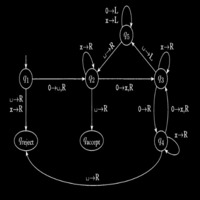
\includegraphics{Im_1.jpg}
    \end{center}
    \newline
    En este diagrama, la etiqueta $0\rightarrow \sqcup,R$ que aparecé en la transición del estado $q_{1}$ al estado $q_{2}$,
    tiene la semántica de la definición de la función $\delta$, que en otras palabras se describe como si:\newline
    en el estado $q_{1}$ con el cabezal leyendo $0$, la máquina va al estado $q_{2}$, escribe $\sqcup$ y mueve el cabezal
    a la derecha.\newline
    Lo cúal en términos formales significa que: $\delta(q_{1},0) = (q_{2},\sqcup, R)$.
    Otra escritura que usaremos para hacer la notación en este ejemplo mas compacta,
    es denotar: $0\leftarrow R$, que la semántica es que se hace la transición del estado $q_{3}$ al estado $q_{4}$, que
    es la etiqueta que se aprecia en el diagrama de estados, y ademas significa que la máquina se mueve a la derecha en
    el momento en el que lee un $0$ en el estado $q_{3}$, pero que no altera la cinta(\no hace una operación escritura),
    entonces $\delta(q_{3}),0) = (q_{4},0,R)$ en términos del mapeo que se esta generando.\newline
    Esta máquina inicia escribiendo un simbolo blanco sobre el último $0$ de lado izquierdo. En particular esto sirve
    para delimitar el final de la cinta con el simbolo blanco $\sqcup$, en esta particular máquina de Turing.
    \newline
    Ahora vamos a hacer una ejecución de esta maquina, $M_{2}$ con la entrada $w = 0000$, en el cual escribiremos la función
    transición $\delta$ con la semántica de las configuraciones.

    %!Here we can use the next sessions of the rows as we can see
    La siguiente secuencia es la ejecución de $M_{2}$ con la entrada en particular $w = 0000$,
    Se lee hacía abajo de las columnas de izquierda a derecha.

    \begin{center}
        \begin{tabular}{c c c}
            $q_{1}0000$ &     $\sqcup q_{5}x0x\sqcup$ & $\sqcup xq_{5}xx\sqcup$ \\
            $\sqcup q_{2}000$ & $q_{5}\sqcup x0x\sqcup$ & $\sqcup q_{5}xxx\sqcup$\\
            $\sqcup xq_{3}00$ & $\sqcup q_{2}x0x\sqcup$ & $q_{5}\sqcup xxx\sqcup$\\
            $\sqcup x0q_{4}0$  & $\sqcup xq_{2}0x\sqcup$ &   $\sqcup q_{2}xxx\sqcup$\\
            $\sqcup x0xq_{3}\sqcup$ & $\sqcup xxq_{3}x\sqcup$ & $\sqcup xq_{2}xx\sqcup$ \\
            $\sqcup x0q_{5}x\sqcup$ & $\sqcup xxxq_{3}\sqcup$ & $\sqcup xxq_{2}x\sqcup$ \\
            $\sqcup xq_{5}0x\sqcup$ & $\sqcup xxq_{5}x\sqcup$ & $\sqcup xxxq_{2}\sqcup$ \\
                            &                                 & $\sqcup xxx\sqcup q_{accept}$ \\
        \end{tabular}
    \end{center}


    %! Final del ejemplo de la máquina de Turing.Inicio de la teoria de Computo Distribuido.
    %! TODO: Hacer la solución gramatical en el siguiente capitulo.
    \section{Decidibilidad en el modelo de computo distribuido  \textbf{LOCAL}}\label{sec:decidibilidad-en-el-modelo-de-computo-distribuidotextbf}
    Ahora lo que haremos es definir el modelo de computo distribuido de manera formal,
    y tomar un modelo en particular en la que enfocaremos nuestro estudio, para posteriormente
    estudiar la noción de decibilidad en dicho modelo.\newline

    En este modelo presentaremos las partes que lo conforman, todo ello de manera formal para ello
    haremos uso de elementos de computo teorico, a priori esto se podra ver como una gráfica donde cada
    nodo se puede representar como una máquina de estados.


    %!Aqui las correcciones que hemos hecho son ese ncialmente triviales

    \subsection{Presentación del modelo de computo distribuido}\label{subsec:presentación-del-modelo-de-computo-distribuido}
    \subsubsection{Presentación del protocolo de comunicación}
    Este modelo tendrá una capa de abstracción de comunicación, asi como su respectiva capa de
    computación de la siguiente manera.
    \subsubsection{Capa de comunicación}
    El modelo de comunicación consiste en una red de comunicación 1-1 que será descrita en términos formales por
    una gráfica conexa, no dirigida $G=(V,E)$, donde los vertices $V=\{ v_{1},\mathellipsis v_{n} \}$,\space
    operando entre ellos.
    Inicialmente, consideraremos identificadores unicos asignados a los procesos de la gráfica $G$.\space
    Más concretamente consideraremos a estos identificadores de un conjunto ordenado de enteros:
    de la siguiente manera:

    \begin{equation}
        S = \{ s_{1},\mathellipsis,s_{n}\} \
        donde:\ s_{i} < s_{i+1} \ \forall i\geq 1\label{eq:equation}
    \end{equation}
    Entonces con esta notación, una ID-asignación es un mapeo:
    $ID:V\rightarrow S$, entonces nos referiremos a su identificador como:
    $ID(v)$. \newline
    Entonces la comunicación se llevara acabo de la siguiente manera: \newline
    Cada vertice tendra asociado el numero de puertos, como el $deg_{G}(v)$,
    entonces en este sentido, el conjunto de aristas adyacentes al vertice
    contiene exactamente $deg_{G}(v)$, donde cada arista esta conectado en un puerto de $v$.
    \newline
    Podemos denotar que a cada arista $(u,v)$ le corresponde la pareja
    $((u,i),(v,j))$, donde $1\leq i \leq deg_{G}(u) $ y $1\leq j \leq deg_{G}(v)$,
    con semántica:\newline \textbf{un canal de comunicación conectadose en el puerto $i$  de $u$ con el puerto $j$ de
    $v$.}\newline
    El vertice $u$ envía(ejecuta la operación $send()$) un mensaje a sus vecinos $v$, cargando el mensaje en un puerto apropiado, digamos $i$.
    Este mensaje es recibido($deliver()$) por $v$, a tráves del puerto $j$. \newline
    %!Aqui se ha acaabado las correcciones de la capa de comunicacion.

    %!Inicio de las correcciones de la capa de computacion.
    \subsubsection{Capa de Computación}
    Una vez que tenemos la capa de comunicación, presentaremos la capa formal del modelo de
    computo.\newline
    El modelo estara governado por un algoritmo $\Pi$, que estará compuesto de protocolos
    $\Pi_{1},\mathellipsis,\Pi_{n}$, donde cada $\Pi_{i}$ residirá en su correspondiente $v_{i}$.
    \newline
    \begin{remark}
        Hasta ahora hemos hablado a secas de los vertices, pero podemos darle una semántica
        de computo en términos de \textbf{procesos}, el cual significa que es una entidad de computo, y entonces a cada $v_{i}$
        lo nombraremos como el proceso $p_{i}$.\newline
        Con esta convención podemos decir que cada protocolo(algoritmo local) $\Pi_{i}$ residirá en su respectivo proceso:
        $p_{i}$.

    \end{remark}
    %!Aqui haremos el entendimiento computacional de los procesos.
    \begin{remark}
        Podemos observar que podemos modelar a cada $\Pi_{i}$ como una maquina de estado para $\forall i$ con su
        correspodiente conjunto de estados estado $Q_{i}$ conteniendo en particular a su estado inicial  $q_{0i}$, asi como sus estados de
        aceptación y rechazo: $q_{accept},q_{reject}\in Q_{i}$, respectivamente tal que en cualquier
        momento dado el proceso $p_{i}$ esta en el estado $q_{i}$ de $Q_{i}$.
        \space
        Mas aún, podemos pensar en cada $\Pi_{i}$ como en una máquina de Turing, equipada con operaciones de envío y
        recepción de \textbf{mensajes}.
    \end{remark}
    %!Lo anterior nos da el preambulo de ver a cada algo como una maquina de Turing.
    \newline
    Por otro lado en la capa de comunicación, tendremos el siguiente esquema:
    \newline
    %!Aqui vamos a dar una definición formal de lo que es un mensaje en un
    %!Manejador de contexto.
    \begin{definition}
        Vámos a definir un mensaje $MSG$ como la información local que sera enviada del proceso $v$ al proceso $u$,
        por medio del canal $((v,i),(u,j))$, donde el proceso $v$ tiene el atributo de la operacion $send(MSG)$, y el vertice
        $v$ hace una operación $deliver(MSG)$, para que finalmente el proceso $v$, hagá una operación $compute()$.
        \newline
        Podemos decir que el tamaño de la información del mensaje $MSG$, es $O(\log n)$ bits.
    \end{definition}

    En cualquier momento dado y en cualquier canal de comunicación $e_{i}=(u,v)$ está en algun estado
    $\overline{q}_{i}$ del conjunto de estados $\overline{Q}_{i}$
    el estado $\overline{q}_{i}$ esta compuesto de dos componentes denotadas de la siguiente manera:
    $\overline{q}_{u\leftarrow v}$ y $\overline{q}_{v\leftarrow v}$ una por cada direccion del canal
    de comunicación.
    Vamos a denotar como $M$ a la colección de todos los posibles mensajes que se pueden enviar de un proceso a otro en toda ejecucion del algoritmo,
    \space cada uno de los dos componentes $\overline{q}_{u \leftarrow v}$ es un elemento de $M \cup \lambda$,
    $\overline{q}_{u\leftarrow v} = MSG\in M$ significa que ahora el mensaje $MSG$ esta en transicion de
    $u$ a $v$, y denotaremos que $\overline{q}_{u\leftarrow v} = \lambda$ para representar una semantica de que
    el canal actual esta vacio en esa dirección.
    En el inicio del computo, todos los procesos estan en el estado inicial $q_{0,i}$ $\forall i$
    y todos los canales de comunicación estan vacios.
    Es decir que sintacticamente: $\overline{q}_{i,0} = <\lambda,\lambda>$
    \newline
    \subsubsection{Ejecución de un algoritmo en este modelo}
    La ejecución del algoritmo en este ambiente consistira de \textbf{Eventos}, ocurriendo en diversos
    lugares de la red y afectando a los procesos involucrados.
    Diremos que un \textbf{paso computacional} es una operación como máquina de Turing del proceso $p$.
    Los eventos puede ser del tipo:
    \begin{itemize}
        \item Computacional: Representando un paso en un procesador
        \item Comunicación: Representando la entrega o la recepción de un mensaje.
    \end{itemize}
    Donde cada evento de comunicación tiene una semántica de:\newline
    $SEND(i,j,MSG)$ o $DELIVER(i,j,MSG)$ para algún mensaje $MSG$.
    Entonces a manera de reportorio de eventos tenemos:
    \begin{enumerate}
        \item Evento $COMPUTE(i)$:\space El proceso $v_{i}$ ejecuta una operación interna, basado en su estado local, y
        posiblemente cambie su estado local.
        \item Evento $SEND(i,j,MSG)$:\space El proceso $v_{i}$ envia de salida un mensaje $MSG$ en algún canal de
        comunicación link $e_{l}$ con destino al proceso $v_{j}$
        \item Evento $DELIVER(i,j,MSG)$:\space El mensaje $MSG $ originado de un proceso $v_{i}$
        que es enviado por el canal de comunicación $e_{l}$ es entregado en la entrada del destino $v_{j}$
    \end{enumerate}
    Entonces la computación en un sistema distribuido lo podemos pensar de la siguiente manera: \newline
    Como una secuencia de configuraciones, capturando el estado actual de los procesos y los canales de comunicación.\newline
    Cada evento cambia de estado para algun procesador $v_{i}$, y posiblemente también para un canal de comunicación
    y eso cambiara la configuracion del sistema.
    En términos formales lo podemos pensar de la siguiente manera:
    \theoremstyle{definition}
    \begin{definition}
        Una \textbf{configuración} es una tupla $(q_{1},\mathellipsis,q_{n},\overline{q}_{1},\mathellipsis,\overline{q}_{m})$,
        donde $q_{i},\overline{q}_{j}$ es el estado del procesador $p_{i}$ y del canal de comunicación $e_{j}$ respectivamente
        y la configuración inicial es:
        \begin{equation}
        q_{0,1},\mathellipsis,q_{0,n},\overline{q}_{0,1},\mathellipsis \overline{q}_{0,m}\label{eq:equation5}
        \end{equation}

        \begin{remark}
            Como estamos pensando de manera intuitiva a cada uno de los procesos como una máquina de Turing, entonces
            una vez que uno de los procesos entra en alguno de los estados:\space $q_{accept},q_{reject}$, el proceso ya no cambía
            de estado, pero sus operaciones de envio y recepción de mensajes siguen activos, i.e quedan activos las
            operaciones de $send(),receive()$.
        \end{remark}
        \newline
        Entonces modelaremos la computación del algoritmo como una (posible) infinita secuencia de configuraciones
        alternadamente con eventos.
    \end{definition}
    \theoremstyle{definition}
    \begin{definition}
        La ejecución de un algoritmo $\Pi$ en una grafica con cierta topología
        $G$, con una entrada inicial $I$ en los procesos es denotado como $\kappa_{\Pi(G,I)}$.
        Formalmente, una \textbf{ejecución} es una secuencia de la forma:
        \begin{equation}
            \kappa = (C_{0},\rho_{1},C_{1},\rho_{2},C_{2},\mathellipsis)\label{eq:equation3}
        \end{equation}
        donde cada $C_{k}$ es una configuración y cada $\rho_{j}$ es un evento,
        y en particular $C_{0}$ denota la configuración inicial.
    \end{definition}
    Podemos imponer ciertas restricciones en las ejecuciones del algoritmo, pero por el momento
    podemos definir formalmente el concepto $\modelo$ en terminos de ejecuciónes para algun algoritmo
    $\Pi$.\newline
    Entonces lo anterior nos permite definir lo siguiente:
    \begin{definition}
        Diremos que un \textbf{modelo} es un subconjunto de esas posibles ejecuciones
    \end{definition}
    Con la definición anterior, nos basaremos en un modelo en particular con una propiedad en particular, a saber el que
    tiene una estructura de rondas.\newline
    \begin{definition}
        Diremos que un \textbf{modelo} tiene el atributo de \textbf{rondas}:
        Si las ejecuciones tienen estructura de \textbf{rondas}, es decir:
        \begin{enumerate}
            \item Cada proceso $p$ ejecuta \textbf{send} a todos sus vecinos, \textbf{deliver} de todos sus vecinos y finalmente \textbf{compute},
            \item Cada proceso ejecuta su $r$-ésima ronda si todos los procesos ejecutaron su $r-1$ ronda.
        \end{enumerate}
    \end{definition}\newline
    La definición anterior nos permitira definir el siguiente modelo:
    \begin{definition}
        Llamaremos \textbf{LOCAL} al modelo que tenga el atributo de \textbf{rondas}
    \end{definition}
    Y podemos observar que el punto 2 de la definición de rondas, es la que da el cáracter de
    síncronia en la ejecución.
    %!Aqui lo que haremos es hacer es tratar de ser lo más claro en las nociones
    %!Enunciados
    \subsubsection{Ejemplos}
    %!todo:Pegar el ejemplo del algoritmo en LOCAL para la versión final de la tesis.


    \newpage
    \subsection{Decidibilidad}\label{subsec:decidibilidad}
    Una vez que tenemos los elementos del modelo distribuido, podemos introducir la noción de \textbf{decibilidad}, en
    este modelo de computo formal.

    \theoremstyle{definition}
    \begin{definition}
        Sea $w$ una cadena, podemos escribir a la cadena como $w_{0},\mathellipsis, w_{n}$, la cual sera la entrada al algoritmo
        $\Pi(w)$, donde de manera distribuida, tendremos como inicialización, que cada proceso $p$ tendra como entrada un caracter de la cadena $w$, digamos $p_{j}(w_{k})$.\newline
        Sea $\kappa_{\Pi(w,G)}$ una ejecución del algoritmo $\Pi$ con entrada $w$ en la grafica $G$, entonces diremos que
        la entrada $w$ es aceptada, si existe una configuración en la ejecución $\kappa_{\Pi(w,G)}$, digamos $C_{k}$ tal que
        existe un estado $q_{a}$ en $C_{k}$, de su correspondiente proceso $p_{a}$, tal que $q_{a}=q_{accept}$.\newline
        Es decir, que el estado en esa configuracion es exactamente el estado $q_{accept}$.\newline
        En simbolos:
        \begin{equation}
            \forall \kappa_{\Pi(w,G)},\ \exists C_{K}\ \mid \exists p_{a}\ \mid q_{a,k}=q_{accept}.\label{eq:equation4}
        \end{equation}
    \end{definition}

    %!--En otras palabras lo que quiere decir es lo siguiente --!%
    Lo anterior, nos permitira definir lo siguiente:
    \begin{definition}
        Al conjunto de cadenas que acepta un algoritmo distribuido $\Pi$ es el lenguaje
        de $\Pi$, o el lenguaje que decide $\Pi$, y lo denotaremos como $L(\Pi)$.
    \end{definition}


    %todo:Migrate the chapter to another file .tex e incluirlo en un main .tex
    \chapter{Simulación de modelos Maquina de Turing y \textbf{LOCAL}}\label{ch:simulacion-de-modelostextbfytextbf}
    \section{Noción de simulación en modelos}\label{sec:nocion-de-simulación-en-modelos}
    Una vez que tenemos estos dos modelos de computo formal, a nivel logico podemos decir que:
    \theoremstyle{definition}
    \begin{definition}
        Decimos que un modelo de computo formal $T$ simula a un modelo de computo formal  $S$ si:
        \begin{equation}
        \forall x\in L(S) \ entonces \ x\in L(T)
        \end{equation}
        Mas aún decimos que son modelos equivalentes (computacionalmente) si:
        \begin{equation}
        \forall x\in L(T) \iff x\in L(S) \
        \end{equation}
    \end{definition}
    \space
    Entonces enunciaremos nuestro teorema de la siguiente manera:

    \begin{theorem}
        Sea $TM$ una maquina de Turing, entonces existe un $\Pi$ algoritmo distribuido que simula
        a $TM$,\space con la semántica de \textbf{simulación}, con base a la definición anterior.
    \end{theorem}
    Una vez que tenemos enunciado este teorema, nos adentraremos al diseño del algoritmo distribuido,
    digamos $\Pi$, tal que para toda ejecucion $\Theta_{\Pi(w,G)}$ con ambiente el modelo \textbf{LOCAL}, con la entrada $w$, para una grafica $G$ con una
    cierta topología, es tal que \textbf{acepta}.
    \newpage

    \section{Diseño del algoritmo}\label{sec:diseño-del-algoritmo}
    \begin{remark}
        Trivialmente, podemos pensar que al darle la entrada la cadena que es aceptada por una maquina de Turing $TM$,\space
        es consumida tal que cada proceso la tiene enteramente como entrada, i.e $\Pi(w)$ entonces de manera local se da
        que $p_{j}(w),\ \forall v_{j}$, entonces este proceso en particular es tal que en algún momento de la ejecución(para alguna ejecució $\Theta_{\Pi(w,G)}$),
        exista una configuración $C_{k}$, y en esta exista un estado $q_{r,k}$, tal que $q_{r,k} = q_{accept}$, pues su respectivo proceso $p_{r}$ es una máquina de Turing,
        por lo tanto de manera global, $w\in L(\Pi)$, pero podemos observar que la forma de la entrada en el algoritmo $\Pi$
        es de manera no distribuida, pues de manera intuitiva todos los procesos saben toda la información.
    \end{remark}
    Entonces no es verdaderamente un diseño de un algoritmo distribuido, por lo tanto procederemos a diseñar de manera
    distribuida el siguiente algoritmo:
    \newline
    %Una vez que tenemos esta información daremos una capa de adversario tal y como lo haremos de esta manera
    %En esta parte daremos una part externa que es la noción de rival en el siguiente sentido
    Daremos la distribución de la información a manera de contricante de la siguente manera:\newline
    Sea $w\in L(TM)$, para una maquina de Turing $TM$ arbitraria, entonces decimos que una rebanada de la cadena
    $w[i]$ o con notación de indice $w_{i}$ tiene localidad $i$.\newline
    Esta semántica nos va a permitir definir lo siguiente:
    \theoremstyle{definition}
    \begin{definition}
        Sea $p_{k}$ un proceso de una grafica $G$, con cierta topología, entonces
        diremos que tendrá una familia $f_{k}$ de posibles entradas, formada por caracteres $w_{t}$, con $t$ localidad para un algoritmo
        distribuido $\Pi$, con ambientación en modelo \textbf{LOCAL}

    \end{definition}
    Esto nos da la noción del control externo de las entradas, que por el momento esto nos esta generando
    una cierta familiaridad del papel a un alto nivel de la visión del contrincante, como podremos observar
    esta es la contraparte del algoritmo que esta gobernando computacionalmente (o por la capa de computo)
    del algoritmo.
    \space
    Entonces nos propondremos el siguiente diseño del algoritmo que nos dará a priori
    la solución del problema que estamos atacando.

    %!---Esta es el diseño sin las definiciones anteriormente enunciadas --!%
    %!---Esto por la nocion del adversario que hemos enunciado anteriormente ---!%
    \begin{algorithm}
        \caption{$Simula\char95Algo\char95TM(w)$}\label{alg:simula}
        \begin{algorithmic}
               %!--Aqui estamos mapeando cada evento del tipo Comp con cada ronda ---!%
               \FORALL{$round \gets 1$}
                  \STATE $v_{j}(w_{i})$\COMMENT{Código para $v_{j}$}
                  \STATE \textbf{read($w_{i}$)}
                  \WHILE{\textbf{true}}
                     \STATE \textbf{call} $\delta(q_{j},w_{i})$
                     \STATE $(q_{r},w_{r},P)\gets \delta(q_{j},w_{i})$
                  \ENDWHILE
                  \IF{$q_{r}==q_{accept}$}
                     \RETURN{$q_{r}$}
                  \ENDIF
                  \ELSE
                       \STATE $MSG\gets<q_{r},w_{r}>$
                       \STATE $\textbf{send}(MSG)$ \textbf{to} $Neighbours(j)$ \COMMENT{vecinos de $j$}
               \ENDFOR
        \end{algorithmic}
    \end{algorithm}
    \space
    %!--El siguiente capitulo es la descripción del algoritmom ----!%
    \section{Descripción del algoritmo}\label{sec:descripción-del-algoritmo}
    Observando el pseudocódigo del algoritmo, podemos observar que vamos a hacer la iteracion por rondas, $round$, en
    virtud del ambiente \textbf{local}, entonces hacemos el código para cada proceso $v_{k}$, luego hacemo la lectura de
    la entrada $w_{i}$, que es la que es por la inicializacion o despues de una operación $deliver(MSG)$, luego hacemos una
    iteración, en la cual haremos llamadas de $\delta()$, y actualizaremos la salida de dicho llamado, para repetir este
    proceso hasta que la localidad de la cadena de salida $w_{r}$, sea de localidad no asignada a la familia de caracteres
    de la cadena, asignada a el proceso actual, el cual es asignado por el lado del contrincate, que es el agente externo del sistema distribuido.
    Finalmente tomamos la decisión de regresar el estado de $q_{accept}$, si el estado $q_{r}==q_{accept}$;
    en otro caso hacemos una operación $send(MSG)$ a los vecinos del proceso actual $v_{k}$.
    \newline
    Lo que sigue, es demostrar que este algoritmo es correcto, lo cual se enunciará en el siguiente teorema.

    \section{Demostración del procedimiento $Simula\char95Algo\char95TM$}\label{sec:demostración-del-procedimiento}
    %!--Primera parte demostrativa del teorema --%!
    \begin{theorem}
        El algoritmo $Simula\char95Algo\char95TM$ es correcto.
    \end{theorem}
    \begin{proof}
        Sea $r$ una ronda de la ejecución del algoritmo $\Pi=Simula\char95Algo\char95TM$,
        al incio de esa ronda se estará iniciando un evento del tipo $COMPUTE(k)$, de nuestro repertorio de eventos para el proceso
        $v_{k}$, por la naturaleza de la distrubución de la información llegara un momento
        de la iteración en la que  se de una estructura de dato $msg\gets <q_{r},w_{r},P>$, arrojada por el llamado iterativo de
        $\delta$, ya que la localidad de $w_{r}$ no esta asignada a $v_{k}$, sin perdida de generalidad.
        Entonces, siguiendo el codigo, observamos que tenemos una lógica para la estructura de dato:
        si $q_{r}==q_{accept}$, entonces $w\in L(\Pi)$, y se acabaria la ejecución en dicha ronda.
        Si no, entonces hacemos la operación $Send(t,MSG)$, donde sin perdida de generalidad $t$ representa el indice de uno de los vecinos
        del proceso $v_{k}$, por otro lado como $w\in L(TM)$ entonces $\exists v_{l}$ en la ronda $r+1$
        tal que al final dicha ronda $\exists q_{l}$ estado tal que $q_{l} == q_{accept}$.\newline
        $\therefore w\in L(\pi)$, por lo tanto el algoritmo es correcto.

    \end{proof}
    Una vez que tenemos la corrección del algoritmo se desprende a manera de corolario la
    simulación de $TM$ en $LOCAL$.
    \begin{corrollary}
        Sea $TM$ una maquina de Turing, entonces:
        \begin{equation}
            \forall w \  \in L(TM) \ \exists \Pi \ algoritmo \ con\ ambientación \ LOCAL\ t.q \ w \in L(\Pi)
        \end{equation}
    \end{corrollary}

    \begin{proof}
        Sean $w\in L(TM)$ para una maquina de Turing y  $\Pi =Simula\char95Algo\char95TM$, $\Pi(w)$ como dicho algoritmo es correcto por el teorema 2,
        entonces ya tenemos un algoritmo  en $LOCAL$ que hace  que $w\in L(w) \ \forall w\in L(TM)$,
        que semánticamente se reduce a que $\Pi$ \textbf{simula} a $TM$, con $TM$ una \textbf{máquina de Turing} abstracta.
    \end{proof}
    %!---Lo que falta es hacer un analisis de complejidad del algoritmo a manera de seccion ---!%

    Entonces una vez que tenemos un algoritmo que es correcto a nivel semantico,
    la siguiente pregunta es la complejidad asociada a la ejecución de $\Pi \gets Simula\char95Algo\char95TM$
    tanto espacial,de comunicación asi como temporal.
    \newpage
    %!---Todo: lo que tenemos que hacer ahora es hacer es una revisión ortograica del doc---!%
    \subsection{Complejidad del algoritmo}\label{subsec:complejidad-del-algoritmo}
    %todo:hacer un main.tex para hacer parte de esta estructura extendible hasta el final de la misma






\end{document}